\subsection{Hadoop Distributed File System}
Das Hadoop Distributed File System ist ein Bestandteil von Hadoop. In diesem Unterkapitel werden die Grundlagen dazu erläutert. Das File System wird definiert und kategorisiert. Außerdem werden die Ziele vom HDFS genannt. Abschließend wird die Architekture erläutert.  
 

\paragraph{Definition}$\;$ \\
Das Hadoop Distributed File System wird definiert als ein \glqq hochverfügbares Dateisystem zur Speicherung sehr großer Datenmengen auf den Dateisystemen mehrerer Rechner (Knoten). Dateien werden in Datenblöcke mit fester Länge zerlegt und redundant auf die teilnehmenden Knoten verteilt. Dabei gibt es Master- und Slave-Knoten. Ein Masterknoten, der so genannte NameNode, bearbeitet eingehende Datenanfragen, organisiert die Ablage von Dateien in den Slaveknoten und speichert anfallende Metadaten. HDFS unterstützt dabei Dateisysteme mit mehreren 100 Mio. Dateien.\grqq (\cite{defhad})

\paragraph{Distributed File Systems}$\;$ \\
Das Hadoop Distributed File System ist ein verteiltes Dateisystem. Ein verteiltes Dateisystem ist ein spezielles Dateisystem, mit dem der Zugriff auf Dateien über ein Rechnernetz erfolgt und das Zugriff und Dateienspeicherung auf mehreren als Server eingesetzten Rechnern erlaubt. Das Gegenstück zu solch einem Netzwerk-Dateisystem ist ein klassisches lokales Dateisystem, welches unmittelbar an den Computer angeschlossene Massenspeicher verwaltet.(vgl.:\cite{distributfs})

\paragraph{Aufgaben von HDFS}$\;$ \\
Normale Distributed File Systems können in bestimmten Situationen unpraktisch sein. Die Dateien lagern auf einer Maschine. Es können nur so viele Dateien auf einer Maschine gespeichert werden, wie die Maschine Speicher frei hat. Ist die Maschine nicht erreichbar, weil es z.B. Netzwerkprobleme gibt, können die Clients keine Dateien aufrufen. Außerdem kann der Zugriff von vielen Clients den Server überfordern.

Das HDFS wurde so konzipiert, dass die Probleme anderer Distributed File Systems, beim Einsatz von HDFS irrelevant sind. HDFS wurde für diesen Einsatzzweck kreeirt. Es ist optimiert für die Speicherung von sehr großen Datenmengen von Informationen. Auch Datenmengen im Bereich von Terabytes oder Petabytes können verarbeitet werden. Die Daten werden über mehrere Maschinen verteilt. Es werden größere Dateiformate als bei normalen Distributed File Systems unterstützt. Die Daten sind auch bei Ausfällen zuverlässig geschützt. Fällt ein Server aus, übernimmt der nächste Sever die Funktion. Das File System skaliert mit der Datenmenge. Werden höhere Datenmengen von vielen Clients angefordert, können weitere Rechner zum Rechnernetz hinzugefügt werden.(vgl.:\cite{yahoo})

Hardware-Defekte passieren regelmäßig. Ein HDFS kann aus mehr als 1000 Maschinen bestehen, wovon jede ein Teil des File System speichert. Da bei der Anzahl von Maschinen anzunehmenen ist, dass nicht jede Maschine problemlos funktionieren wird, verfügt HDFS dafür, über eine automatische Wiederherstellungsfunktion. Das Hadoop Distributed File System ist ausgerichtet für Batchjobs statt für interaktiven Benutzerzugriff. Der Fokus liegt auf einem hohen Datendurchsatz statt auf einer niedrigen Latenz.(vgl.:\cite{archguid})
 
\paragraph{Architektur}$\;$ \\
Im Folgenden wird die Architektur von HDFS beschrieben. Die Architektur ist ausgelegt, für Anwendungsfälle wo Daten einmal ins File System übergeben werden und von dort vielfach ausgelesen werden. Damit die Daten verteilt gespeichert werden können, werden die Daten in Blöcke aufgespalten und auf den Knoten des Hadoop-Clusters verteilt. Für jeder dieser Blöcke werden Kopien auf verschiedenen Servern im Cluster angelegt, um Fehler und Ausfallsicherheit zu garantieren. Das zugehörige Management wird von HDFS übernommen. Der Zugriff auf das HDFS ähnelt Unix. Sowohl Konsolen-Befehle, als auch die Rechteverwaltung der Dateien funktionieren wie bei Unix. 

Die Architektur ist eine Master-Slave-Architektur (Siehe Abbildung:\ref{fig:Architektur}). Die Architektur umfasst dabei verschiedene Komponente, wie Master, Client, NameNode und DataNode. Der Client fordert ein File an vom Server. Der Server ist der Master. Der Master beinhaltet ein NameNode. Das NameNode ist die zentrale Masterkomponente und verwaltet die Metadaten für alle gespeicherten auf allen DataNodes. Im Block Map speichert der Master alle aktuellen Speicherorte der Blöcke von Verzeichnissen und Dateien. Der Master beinhaltet außerdem noch das Journal Log, in dem aktuelle Dateioperationen gespeichert werden. Auf der Grundlage von Block Map und Journal Log, kann der Master Anfragen nach Dateien beantworten. Die DataNodes sind die Slave-Komponenten. Diese sind für die Datenspeicherung zuständig. Soll der HDFS-Cluster vergrößert werden, werden DataNodes hinzugefügt. Der NameNode wird vom Secondary NameNode unterstützt. Der Secondary NameNode entlastet den NameNode beim Zusammenführen und Verarbeiten der Block Map und Journal Log.(vgl.:\cite{uwe})

\begin{figure}[h!]
    \centering
    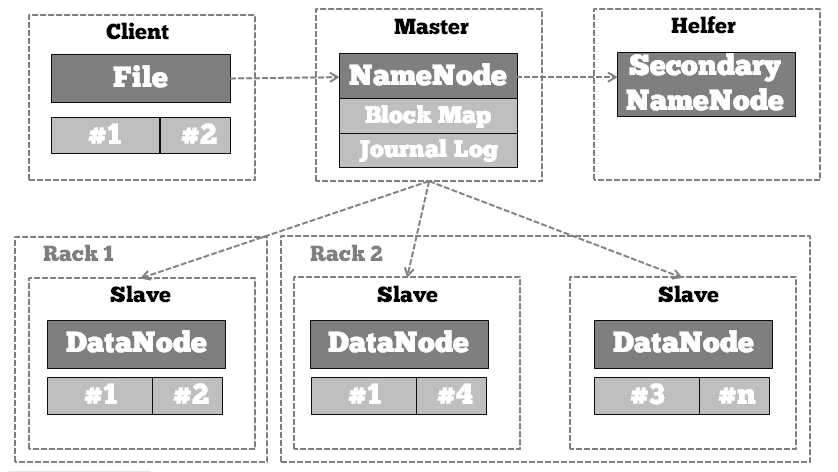
\includegraphics[width=0.55\linewidth]{hha.png}
    \caption{Architektur\cite{uwes}}
    \label{fig:Architektur}
  \end{figure}

  

